\documentclass[10pt]{article}

% amsmath package, useful for mathematical formulas
\usepackage{amsmath}
% amssymb package, useful for mathematical symbols
\usepackage{amssymb}

% graphicx package, useful for including eps and pdf graphics
% include graphics with the command \includegraphics
\usepackage{graphicx}

% cite package, to clean up citations in the main text. Do not remove.
\usepackage{cite}

\usepackage{color} 

% Use doublespacing - comment out for single spacing
%\usepackage{setspace} 
%\doublespacing


% Text layout
\topmargin 0.0cm
\oddsidemargin 0.5cm
\evensidemargin 0.5cm
\textwidth 16cm 
\textheight 21cm

% Bold the 'Figure #' in the caption and separate it with a period
% Captions will be left justified
\usepackage[labelfont=bf,labelsep=period,justification=raggedright]{caption}

% Use the PLoS provided bibtex style
\bibliographystyle{plos2009}

% Remove brackets from numbering in List of References
\makeatletter
\renewcommand{\@biblabel}[1]{\quad#1.}
\makeatother


% Leave date blank
\date{}

\pagestyle{myheadings}
%% ** EDIT HERE **
%\usepackage{bm}

%% ** EDIT HERE **
%% PLEASE INCLUDE ALL MACROS BELOW

%% END MACROS SECTION

\begin{document}

% Title must be 150 characters or less
\begin{flushleft}
{\Large
\textbf{Appendix S1: Optimization details}
}
% Insert Author names, affiliations and corresponding author email.
\\
David L. Miller$^{1,\ast}$,
Len Thomas$^{1}$
\\
\bf{1} School of Mathematics and Statistics, and Centre for Research into Ecological and Environmental Modelling, University of St Andrews, St Andrews KY16 9LZ, Scotland
\\
$\ast$ E-mail: dave@ninepointeightone.net
\end{flushleft}

In practice, maximization is performed on the $\log$-likelihood. However, as noted in the literature \cite{Gelman:2013tc, Marin:2005wf}, mixture model likelihoods can be notoriously multimodal. This can cause problems when finding MLEs of the parameters. Here simulated annealing (SANN; \cite[Chapter 10]{Press:1990tn}) was used to explore the parameter space (for 500 iterations) then after that the Broyden-Fletcher-Goldfarb-Shanno method (BFGS; \cite[Chapter 10]{Press:1990tn}) was used to find the maxima (the implementations in the R function optim() were used). These two steps were run 5 times. This two step approach appears to be satisfactory in most cases. The EM algorithm \cite{Dempster:1977ul} was tested although there was no significant performance increase (in terms of computational time or parameter precision) over using BFGS with SANN. To aid the optimization, analytic derivatives were also used; these are given in Text S2.

\subsection*{Starting values}

Beavers and Ramsay \cite{Beavers:1998wk} give a method for estimating starting values for the scale parameter of a half-normal detection function. In the non-covariate case, the estimate is given as the intercept parameter from intercept only regression on $\log(y+\frac{w}{1000})$ (where $w$ denotes the truncation distance, as above). For covariate models, the equation used for the $\sigma$ is used in the regression and the estimated parameters from the linear regression are used as the starting values for the $\beta$s.

A similar approach can be use in the mixture case by dividing the sorted distances into $J$ equal parts. For each of these parts a Beavers and Ramsay-type estimate is used for the $\beta$s. The mixture weight $\phi_j$ had starting values of $1/J$ since there is no reason \textit{a priori} to believe anything else.

\subsection*{Parametrisation of the mixture proportions}

When using 2-point mixtures, the constraint that the mixture proportions must sum to unity is enforced by definition (since $\phi_2=1-\phi_1$). However, in $J$-point mixtures when $J>2$ ensuring that the proportions sum to 1 is not guaranteed. The obvious way to get around this would be to penalise the likelihood, should the optimisation procedure propose values for the $\phi_j$s that are not in accordance with this condition. This is, of course, inefficient and ugly. Instead, a parametrisation is used for the mixture proportions which yields $\phi_j$s that comply.

Rather than estimating the $\phi_j$s, estimate $\alpha_p$s ($p=1,\ldots,J$), where the relationship between the two is:
\begin{equation*}
\phi_j = F(\sum_{p=1}^j e^{\alpha_p}) - F(\sum_{p=1}^{j-1} e^{\alpha_p}) \qquad \text{for } 1\leq j \leq J-1
\end{equation*}
and
\begin{equation*}
\phi_J = 1-\sum_{j=1}^{J-1} \phi_j
\end{equation*}
where $F$ is any continuous CDF on $(0,\infty]$. Exponentiation ensures that $e^{\alpha_p}\geq0$, so $\alpha_p$ may lie anywhere on the real line, allowing unconstrained optimisation. Summing these orders the $\phi_j$s, since only offsets are estimated. Finally, using the cumulative density function ensures that the $\phi_j$s sum to $1$. In practise the $\text{Gamma}(3,2)$ CDF is (somewhat arbitrarily) used. Figure \ref{mmds-phifig} illustrates the relationship.

\begin{figure*}
\centering
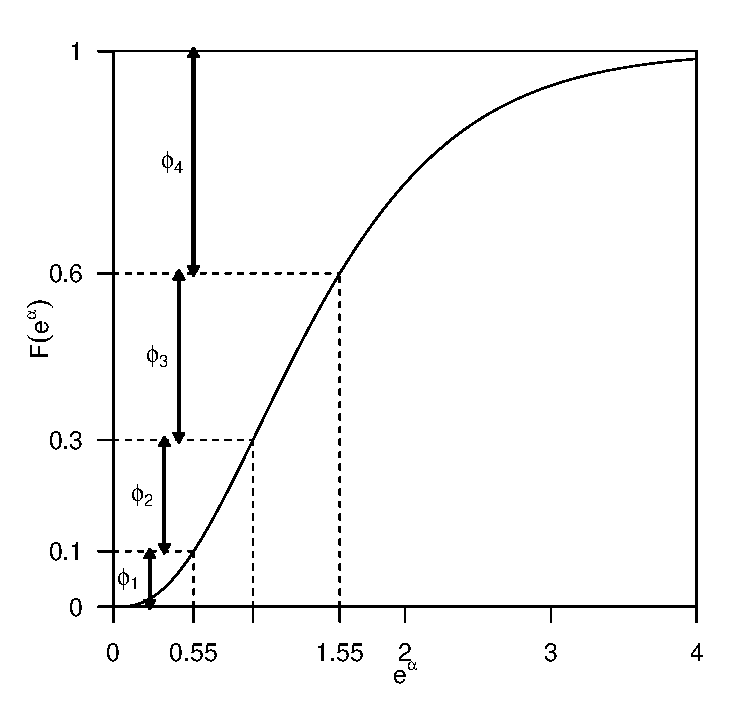
\includegraphics{figs/phidia.pdf}
\caption{The relationship between the mixture proportions, $\phi_j$ and the quantities estimated during the optimization procedure, $\alpha_p$.}
\label{mmds-phifig}
\end{figure*}

To transform from the $\phi_j$s back to the $\alpha_p$s we simply re-arrange the above expression.
\begin{equation*}
\alpha_p = \log_e \Big(F^{-1}\Big(\phi_j + F(\sum_{p=1}^{j-1} e^{\alpha_p})\Big) - \sum_{p=1}^{j-1} e^{\alpha_p}\Big).
\end{equation*}
Note that we only need as many $\alpha_p$s as we had $\phi_j$s, so we do not require any additional parameters.


\bibliography{dsmixtures-appendix}

\end{document}